\section{Threads}
parallel ablaufende Aktivitäten innerhalb Prozess, Geteilte Ressourcen: text section, data section, Heap, geöffnete Dateien, MMU-Infos | jeder Thread eigener Stack + Kontext (da unterschiedliche Stadien, eigene Funktionsaufrufkette)$\rightarrow$Thread-Control Block

\subsection{Amdahls Regel}
\begin{description}
\item[$\textcolor{green}{n}$]Anzahl Prozessoren
\item[$\textcolor{red}{T}$]Ausführungszeit, wenn komplett seriell ausgeführt
\item[$T'$]Zeit, wenn max. parallelisiert ($\textcolor{brown}{\textcolor{brown}{T_{s}}} + \frac{\textcolor{red}{T}-\textcolor{brown}{\textcolor{brown}{\textcolor{brown}{T_{s}}}}}{\textcolor{green}{n}}$)
\item[$\textcolor{brown}{\textcolor{brown}{\textcolor{brown}{T_{s}}}}$]Zeit, der seriell ausgeführt werden muss
\item[$\textcolor{red}{T} - \textcolor{brown}{\textcolor{brown}{\textcolor{brown}{T_{s}}}}$]Zeit, die parallisiert werden kann
\item[$\frac{\textcolor{red}{T} - \textcolor{brown}{\textcolor{brown}{\textcolor{brown}{T_{s}}}}}{\textcolor{green}{n}}$]Parallel-Anteil verteilt auf n Prozessoren
\item[$\textcolor{blue}{s} = \frac{\textcolor{brown}{T_s}}{\textcolor{red}{T}}$]serieller Anteil Algorithmus
\end{description}

\subsubsection{Speedup-Faktor}
$f \le \frac{\textcolor{red}{T}}{T'} = \frac{\textcolor{red}{T}}{\textcolor{brown}{\textcolor{brown}{\textcolor{brown}{T_{s}}}} + \frac{\textcolor{red}{T} - \textcolor{brown}{\textcolor{brown}{\textcolor{brown}{T_{s}}}}}{\textcolor{green}{n}}} = \frac{\textcolor{red}{T}}{\textcolor{blue}{s} \cdot \textcolor{red}{T} + \frac{\textcolor{red}{T}-\textcolor{blue}{s}\cdot \textcolor{red}{T}}{\textcolor{green}{n}}} = \frac{\textcolor{red}{T}}{\textcolor{blue}{s} \cdot \textcolor{red}{T} + \frac{1-\textcolor{blue}{s}}{\textcolor{green}{n}} \cdot \textcolor{red}{T}} = \frac{1}{\textcolor{blue}{s} + \frac{1-\textcolor{blue}{s}}{\textcolor{green}{n}}}$\\
parallele Variante max. $f$-mal schneller als serielle

\subsubsection{Bedeutung}
\begin{multicols*}{2}
Abschätzung einer oberen Schranke/max. Geschwindigkeitsgewinn\\
Nur wenn alles parallelisierbar ist, ist Speedup proportional und maximal $f(\textcolor{blue}{0},\textcolor{green}{n}) = \textcolor{green}{n}$\\
Sonst Speedup mit höherem $\textcolor{green}{n}$ geringer\\
\columnbreak
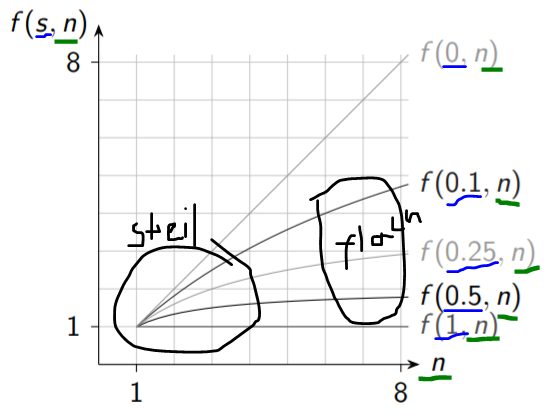
\includegraphics[scale = 0.35]{grafiken/amdahl_graph.PNG}
\end{multicols*}

Mit höherer Anz. Prozessoren nähert sich Speedup $\frac{1}{\textcolor{blue}{s}}$ an: $lim\limits_{\textcolor{green}{n} \to \infty}\frac{1}{\textcolor{blue}{s} + \frac{1-\textcolor{blue}{s}}{\textcolor{green}{n}}} = \frac{1}{\textcolor{blue}{s}}$

\subsection{POSIX Thread API}
\begin{minted}{c}
int pthread_create (
pthread_t * thread_id, //Out-Parameter
pthread_attr_t const * attributes, //0 -> default
void * (* start_function ) ( void *) ,//1. Instruktion v. Thread
void * argument )//Argumente an Funktion, Pointer auf Heapobj.
\end{minted}
Attribut angeben, Vorgehensweise:
%\begin{minted}{C}
%pthread_attr_t attr ;
%pthread_attr_init (& attr );
%pthread_attr_setstacksize (& attr , 1 << 16);
%pthread_create (... , & attr , ...);
%pthread_attr_destroy (& attr );
%\end{minted}
\textbf{Lebensdauer/Beendigung Threat: }springt aus \prgc{start_function} zurück, ruft \prgc{pthread_exit} auf, anderer Thread ruft \prgc{pthread_cancel} auf, Prozess wird beendet\\
\prgc{void pthread_exit(void * return_value)//gleicher Wert wie start_function}\\
\prgc{int thread_cancel(pthread_t thread_id)} 0 = existiert, ESRCH existiert nicht, Funktion wartet nicht bis Thread tatsächlich beendet wurde\\
\prgc{int pthread_detach(pthread_t thread_id)}\\
entfernt Speicher, den Thread belegt hatte aber beendet nicht\\
\prgc{int pthread_join(pthread_t thread_id , void ** return_value)}
Wartet bis Thread beendet, Rückgabe wie create oder exit (0 keine)\\
\prgc{pthread_t pthread_self (void)} ID laufenden Threats


